\begin{frame}{Going further (1): Branches}
  \begin{itemize}
    \item several people can work at the same project at the same time
    \item they might make incompatible changes (that can be united later)
    \item git allows the versions of a repository to diverge using branches
    \inote{they can also be brought back together using merging later}
    \item The default branch is usually called ``master''
    \item Each branch has a so-called HEAD that points to its latest commit
    \item There is also a HEAD of the repository which points to the current branch
  \end{itemize}
\end{frame}

\begin{frame}{Going further (2): Branching \& Merging}
  \begin{columns}[onlytextwidth]
    \begin{column}{0.5\textwidth}
      \begin{itemize}
        \item you can make commits on branches like you would normally
          \inote{but you need to switch to them first}
        \begin{itemize}
          \item \shellcmd{git branch name} - create a branch
          \item \shellcmd{git checkout name} - switch to it
          \item \shellcmd{git merge name} - merge a branch back into the current one
        \end{itemize}
        \item Time for another short demo
      \end{itemize}
    \end{column}
    \begin{column}{0.5\textwidth}
      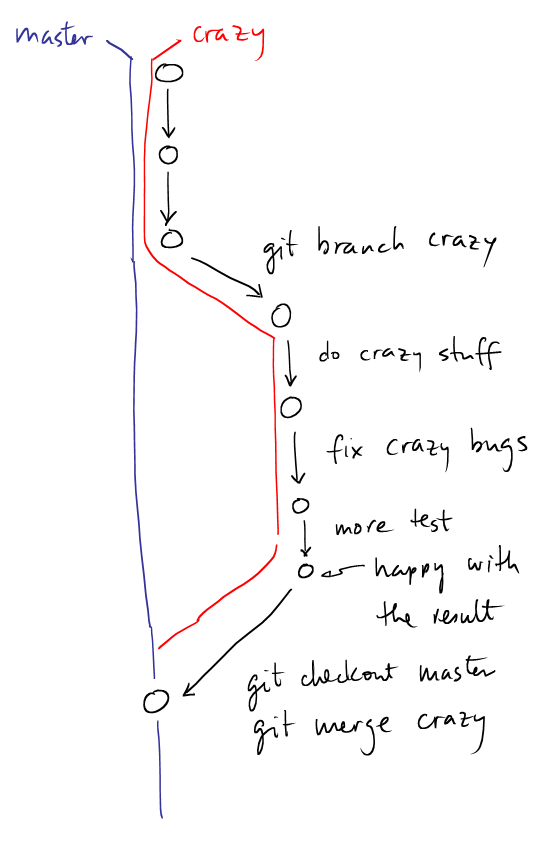
\includegraphics[height=\textheight]{imgs/branches}
    \end{column}
  \end{columns}
\end{frame}

\begin{frame}{Going further (3): Resolving Merge conflicts}
  \begin{itemize}
    \item merging can cause conflicts
    \inote{when files were modified on both branches and git can not merge them automatically}
    \item git will tell you when you run \shellcmd{git merge} if there are conflicts
    \begin{itemize}
      \item you can edit the affected files manually, then stage the files (\shellcmd{git add}) and commit them (\shellcmd{git commit})
      \inote{\shellcmd{git status} is always helpful when doing this}
      \item \shellcmd{git merge --abort} - cancel the merge and go back to what was there before
      \item ``fake'' a merge by forcing git to use one of the two versions
      \begin{itemize}
        \item \shellcmd{git merge -X ours branch} - use the version of the current branch
        \item \shellcmd{git merge -X theirs branch} - use the other branches version
        \item (you need to do this before starting to merge)
      \end{itemize}
    \end{itemize}
  \end{itemize}
\end{frame}

\begin{frame}{Going further (4): Working with remotes}
  \begin{itemize}
    \item a remote is a clone of the same repository in another location
    \inote{usually on a remote server}
    \item you can add and remove remotes dynamically
    \inote{e.g. \shellcmd{git remote add name url}}
    \item when you \shellcmd{git clone} a repository a remote ``origin'' will be added automatically
    \item remotes have branches and you can push and pull your local branches
    \begin{itemize}
      \item \shellcmd{git push remote branch} - pushes the \textit{branch} to the remote \textit{remote}
        \inote{if you use \shellcmd{git push -u} you can just you can omit the names afterwards}
      \item \shellcmd{git fetch remote/branch} - fetches new commits from the remote branch only. 
        \inote{It can happen that only a rebase takes place}
      \item \shellcmd{git pull} - fetches new commits from the tracked branch and merges them into the local branch
    \end{itemize}  
  \end{itemize}
\end{frame}

\begin{frame}{Going further (5): Common Practices for Pushing \& Pulling}
  \begin{columns}[onlytextwidth]
    \begin{column}{0.7\textwidth}
      \begin{itemize}
        \item if you clone a repository, you usually only need \shellcmd{git push} and \shellcmd{git pull}
        \item before pushing new commits you need to pull first
          \inote{there is \shellcmd{git push --force} but you {\huge never} want to do this because this can lead to loss of data. }
        \item when pulling new commits, merge conflicts might occur
          \inote{use \shellcmd{git fetch remote/branch} and then \shellcmd{git merge remote/branch} to resolve conflicts}
      \end{itemize}
    \end{column}
    \begin{column}{0.3\textwidth}
      
\includegraphics[width=0.9\textwidth]{imgs/no_force}
    \end{column}
  \end{columns}
\end{frame}

\begin{frame}{Going further (5): Common Practices for Pushing \& Pulling}
  \begin{columns}[onlytextwidth]
    \begin{column}{0.7\textwidth}
      \begin{itemize}
        \item if you clone a repository, you usually only need \shellcmd{git push} and \shellcmd{git pull}
        \item before pushing new commits you need to pull first
          \inote{there is \shellcmd{git push --force} but you {\huge never} want to do this because this can lead to loss of data. }
        \item when pulling new commits, merge conflicts might occur
          \inote{use \shellcmd{git fetch remote/branch} and then \shellcmd{git merge remote/branch} to resolve conflicts}
      \end{itemize}
    \end{column}
    \begin{column}{0.3\textwidth}
      
\includegraphics[width=0.9\textwidth]{imgs/no_force}
    \end{column}
  \end{columns}
\end{frame}

\begin{frame}{Going further (6): Other useful commands}
  \begin{itemize}
    \item \shellcmd{git diff} - to see unstaged changes inside files
    \item \shellcmd{git log} - show a log of recent commits on the current branch
      \inote{exit by pressing \textit{q}}
    \item \shellcmd{git commit --amend} - Edit the previous commit instead of creating a new one. 
    \item \shellcmd{git reset HEAD files} - removes changes from the staging area
    \item \shellcmd{git stash} - Stash your changes for a rainy day
    \item \shellcmd{git tag} - give names to certain commits
    \item \dots
  \end{itemize}
\end{frame}